\documentclass{sig-alternate}
%\usepackage[latin1]{inputenc} % Windows
\usepackage[utf8x]{inputenc} % Linux (unicode package needed)
% \usepackage[applemac]{inputenc} % Mac

\usepackage{hyperref}

\usepackage{balance}

\usepackage{graphicx}
\usepackage{caption}
\usepackage{subcaption}
\usepackage{hyperref}

\usepackage{xcolor}
\usepackage{color}

\newcommand{\brand}[1]{\textbf{\tt #1}}

\usepackage{enumitem}
\setlist[description]{leftmargin=\parindent}

\definecolor{editorGray}{rgb}{0.95, 0.95, 0.95}
\definecolor{editorOcher}{rgb}{1, 0.5, 0} % #FF7F00 -> rgb(239, 169, 0)
\definecolor{editorGreen}{rgb}{0, 0.5, 0} % #007C00 -> rgb(0, 124, 0)
\colorlet{punct}{red!60!black}
\definecolor{background}{HTML}{F5F5F5}
\definecolor{delim}{RGB}{20,105,176}
\colorlet{numb}{magenta!60!black}

\usepackage{upquote}
\usepackage{listings}
\lstdefinelanguage{JavaScript}{
  morekeywords={typeof, new, true, false, catch, function, return, null, catch, switch, var, if, in, while, do, else, case, break},
  morecomment=[s]{/*}{*/},
  morecomment=[l]//,
  morestring=[b]",
  morestring=[b]'
}

\lstdefinelanguage{HTML5}{
        language=html,
        sensitive=true, 
        alsoletter={<>=-},
        otherkeywords={
        % HTML tags
        <html>, <head>, <title>, </title>, <meta, />, </head>, <body>,
        <canvas, \/canvas>, <script>, </script>, </body>, </html>, <!, html>, <style>, </style>, ><
        },  
        ndkeywords={
        % General
        =,
        % HTML attributes
        charset=, id=, width=, height=,
        % CSS properties
        border:, transform:, -moz-transform:, transition-duration:, transition-property:, transition-timing-function:
        },  
        morecomment=[s]{<!--}{-->},
        tag=[s]
}

\lstset{%
    % Basic design
    backgroundcolor=\color{background},
    basicstyle={\scriptsize\ttfamily},   
    frame=none,
    % Line numbers
    numbers=none,
    % xleftmargin={0.75cm},
    % numbers=left,
    % stepnumber=1,
    % firstnumber=1,
    % numberfirstline=true,
    % Code design   
    keywordstyle=\color{blue}\bfseries,
    commentstyle=\color{darkgray}\ttfamily,
    ndkeywordstyle=\color{editorGreen}\bfseries,
    stringstyle=\color{delim},
    % Code
    language=HTML5,
    alsolanguage=JavaScript,
    alsodigit={.:;},
    tabsize=2,
    showtabs=false,
    showspaces=false,
    showstringspaces=false,
    extendedchars=true,
    breaklines=true,        
    % Support for German umlauts
    literate=%
    {Ö}{{\"O}}1
    {Ä}{{\"A}}1
    {Ü}{{\"U}}1
    {ß}{{\ss}}1
    {ü}{{\"u}}1
    {ä}{{\"a}}1
    {ö}{{\"o}}1
}

\lstdefinelanguage{json}{
    basicstyle=\scriptsize\ttfamily,
    % Line numbers
    numbers=none,
    frame=none,
    % numbers=left,
    % numberstyle=\scriptsize,
    % stepnumber=1,
    % numbersep=8pt,
    % showstringspaces=false,
    % breaklines=true,
    % frame=lines,
    backgroundcolor=\color{background},
    literate=
     *{0}{{{\color{numb}0}}}{1}
      {1}{{{\color{numb}1}}}{1}
      {2}{{{\color{numb}2}}}{1}
      {3}{{{\color{numb}3}}}{1}
      {4}{{{\color{numb}4}}}{1}
      {5}{{{\color{numb}5}}}{1}
      {6}{{{\color{numb}6}}}{1}
      {7}{{{\color{numb}7}}}{1}
      {8}{{{\color{numb}8}}}{1}
      {9}{{{\color{numb}9}}}{1}
      {:}{{{\color{punct}{:}}}}{1}
      {,}{{{\color{punct}{,}}}}{1}
      {\{}{{{\color{delim}{\{}}}}{1}
      {\}}{{{\color{delim}{\}}}}}{1}
      {[}{{{\color{delim}{[}}}}{1}
      {]}{{{\color{delim}{]}}}}{1},
}

\begin{document}

% Copyright
\setcopyright{acmcopyright}
%\setcopyright{acmlicensed}
%\setcopyright{rightsretained}
%\setcopyright{usgov}
%\setcopyright{usgovmixed}
%\setcopyright{cagov}
%\setcopyright{cagovmixed}


% DOI
\doi{10.475/123_4}

% ISBN
\isbn{123-4567-24-567/08/06}

%Conference
\conferenceinfo{DocEng2015}{Sep 8--11, 2015, Lausanne, Switzerland}

\acmPrice{\$15.00}

\title{x-project: a document-oriented toolkit to design and implement Web Applications based on HTML5 Web Components}

\numberofauthors{4} 
\author{
\alignauthor
Andrea D'Amelio\\
  \affaddr{Universit\`a Roma Tre}\\
  \affaddr{Dipartimento di Ingegneria}\\
  \affaddr{Universit\`a Roma Tre}\\
  \affaddr{Rome, Italy}\\
  \email{damelio@ing.uniroma3.it}
\alignauthor
Enrico Marino\\
  \affaddr{Universit\`a Roma Tre}\\
  \affaddr{Dipartimento di Ingegneria}\\
  \affaddr{Universit\`a Roma Tre}\\
  \affaddr{Rome, Italy}\\
  \email{marino@ing.uniroma3.it}
\and
\alignauthor
Tiziano Sperati\\
  \affaddr{Universit\`a Roma Tre}\\
  \affaddr{Dipartimento di Ingegneria}\\
  \affaddr{Universit\`a Roma Tre}\\
  \affaddr{Rome, Italy}\\
  \email{sperati@ing.uniroma3.it}
\alignauthor
Federico Spini\\
  \affaddr{Universit\`a Roma Tre}\\
  \affaddr{Dipartimento di Ingegneria}\\
  \affaddr{Universit\`a Roma Tre}\\
  \affaddr{Rome, Italy}\\
  \email{spini@ing.uniroma3.it}
}

\maketitle

\begin{abstract}
In this paper a software toolkit named \brand{x-project} is introduced. It consists of a Web Component library which applied over a very powerful web framework, i.e. Loopback by Strongloop, realize an ibrid prototypal tool which bring togheter the customizability of a modern web framework with the ease of use of traditional CMSs.

Furthermore, the introduction of this tool implicitly defines a document-driven development process that extremize the concept of the reuse of code whose complessive readability, maintainability and extendibility result dramaticaly increased.
\end{abstract}


%
% The code below should be generated by the tool at
% http://dl.acm.org/ccs.cfm
% Please copy and paste the code instead of the example below. 
%

\begin{CCSXML}
<ccs2012>
<concept>
<concept_id>10002951.10003260.10003282</concept_id>
<concept_desc>Information systems~Web applications</concept_desc>
<concept_significance>500</concept_significance>
</concept>
<concept>
<concept_id>10010405.10010476.10010479</concept_id>
<concept_desc>Applied computing~Cartography</concept_desc>
<concept_significance>500</concept_significance>
</concept>
<concept>
<concept_id>10010405.10010497.10010510.10010514</concept_id>
<concept_desc>Applied computing~Format and notation</concept_desc>
<concept_significance>500</concept_significance>
</concept>
<concept>
<concept_id>10010520.10010521.10010537.10010538</concept_id>
<concept_desc>Computer systems organization~Client-server architectures</concept_desc>
<concept_significance>300</concept_significance>
</concept>
<concept>
<concept_id>10010520.10010570.10010574</concept_id>
<concept_desc>Computer systems organization~Real-time system architecture</concept_desc>
<concept_significance>300</concept_significance>
</concept>
</ccs2012>
\end{CCSXML}

\ccsdesc[500]{Information systems~Web applications}
\ccsdesc[500]{Applied computing~Cartography}
\ccsdesc[500]{Applied computing~Format and notation}
\ccsdesc[300]{Computer systems organization~Client-server architectures}
\ccsdesc[300]{Computer systems organization~Real-time system architecture}

%
% End generated code
%

%
%  Use this command to print the description
%
\printccsdesc

\section{Introduction}\label{sec:introduction}

Since the beginning of Internet, the ability to create and publish content on the web has made the success of Content Management Systems. Products like \href{http://www.joomla.org/}{Joomla!} or \href{https://wordpress.org/}{WordPress}, born to handle simple websites or blogs, are evolved to support web applications of any sort (from personal portfolio, to on-line newspaper or on-line shopping), running as of January 2015 more than 25\% of the top ten million websites \cite{usage-cms}. This evolution has been allowed by a plug-in based architecture, where each plug-in is responsible to handle a functionality subset of the whole application, presenting the user through a simple accessible configuration and management interface.

The large number of available plug-ins covers most of the common and frequently required customizations, thus avoiding to write ad-hoc code. Nevertheless, the implementation of specific functional characteristics inevitably require to intervene at code level.

When the effort required to add custom features to a CMS results too expensive, a web framework can be adopted instead. A web framework consists of a set of software facilities that aims to alleviate the overhead associate with common development activities. Web application coding effort, while eased by the web framework, is anyway rewarded with an increased level of extensibility and customizability of the resulting application.

The most desirable features for a web framework are: a) user management, b) session management, c) automatic generation of CRUD methods on data models exposed via HTTP RESTfull API, d) data access policies management. In order to effectively speed up web applications development, these facilities should be provided relying mostly on external configuration files and less on procedural code \cite{6859693}.

In this paper a software toolkit named \brand{x-project} is introduced. It consists of a Web Component library that is applied over a very powerful web framework, i.e. Loopback by Strongloop, and realizes an hybrid prototypal tool which brings together the customizability of a modern web framework with the ease of use of traditional CMSs.

Furthermore, the use of the toolkit alongside the web framework implicitly defines a document-driven development process that polarizes the concept of reusing the code whose overall readability, maintainability and extendibility result dramatically increased.

The remainder of this document is organized as follows. Section~\ref{sec:architecture} is devoted to describe the architecture and the technology stack exposed by applications developed by the toolkit, while section~\ref{sec:toolkit} presents the toolkit itself. Section~\ref{sec:dev-proc} outlines the development process implicitly defined by the \brand{x-project} toolkit. Finally section~\ref{sec:case-study} reports about a case-study application: it is shown how the toolkit can be used to build a blog.



\section{Architecture}
\brand{x-project} architecture is client-server.
The full technology stack is JavaScript based.

Server-side is based on Node.js.

\begin{description}
\itemsep1pt\parskip0pt\parsep0pt
        \item[Node.js] (\url{http://nodejs.org}) is a platform built on Chrome's JavaScript runtime for easily building fast, scalable network applications.
        \item[Express.js] (\url{http://expressjs.com}) is a minimal and flexible Node.js web application framework that provides a set of features for web and mobile applications.
        \item[Loopback] (\url{http://loopback.io}) is a set of Node.js modules to develop Web Servers applications. An application interacts with data sources through the LoopBack model API, available locally within Node.js, remotely over REST.
        \item[MongoDB] (\url{https://www.mongodb.org/}) is an open-source document database that provides high performance, high availability, and automatic scaling.
\end{description}


Client-side is based on Web Components.

\begin{description}
\itemsep1pt\parskip0pt\parsep0pt
        \item[Web Components] are a collection of standards which are working their way through the W3C and landing in browsers at the moment. In a nutshell, they allow us to bundle markup and styles into custom HTML elements.
\emph{Custom Elements}\cite{custom-elements}, \emph{HTML Imports}\cite{html-imports}, \emph{HTML Templates}\cite{html-templates}, \emph{Shadow DOM}\cite{shadow-dom}.
        \item[webcomponent.js polyfills] enable Web Components in (evergreen) browsers that lack native support.
Web Components specifications are currently W3C Working Draft, so they aren’t fully supported across all major browsers.
As these technologies are implemented in browsers, the polyfills will shrink to gain the benefits of native implementations. \cite{webcomponents-polyfills} 
        \item[Polymer library] (\url{https://www.polymer-project.org/}) provides a thin layer of API on top of web components (native implementations and their polyfills) and several powerful features, such as custom events and delegation, mixins, accessors and component lifecycle functions, that makes it easier and faster to create Web Components. Similar to \emph{Polymer} are \emph{x-tag} and \emph{Bosonic}.
        \item[iron-elements] \cite{iron-elements} is a library of utility Polymer elements from ajax requests to input elements. 
There are web repositories like \url{http://component.kitchen} and \url{http://customelements.io} that already counts thousands of open source user-contributed custom elements.
\end{description}

% \begin{figure}[!htbp]
% \centering
% 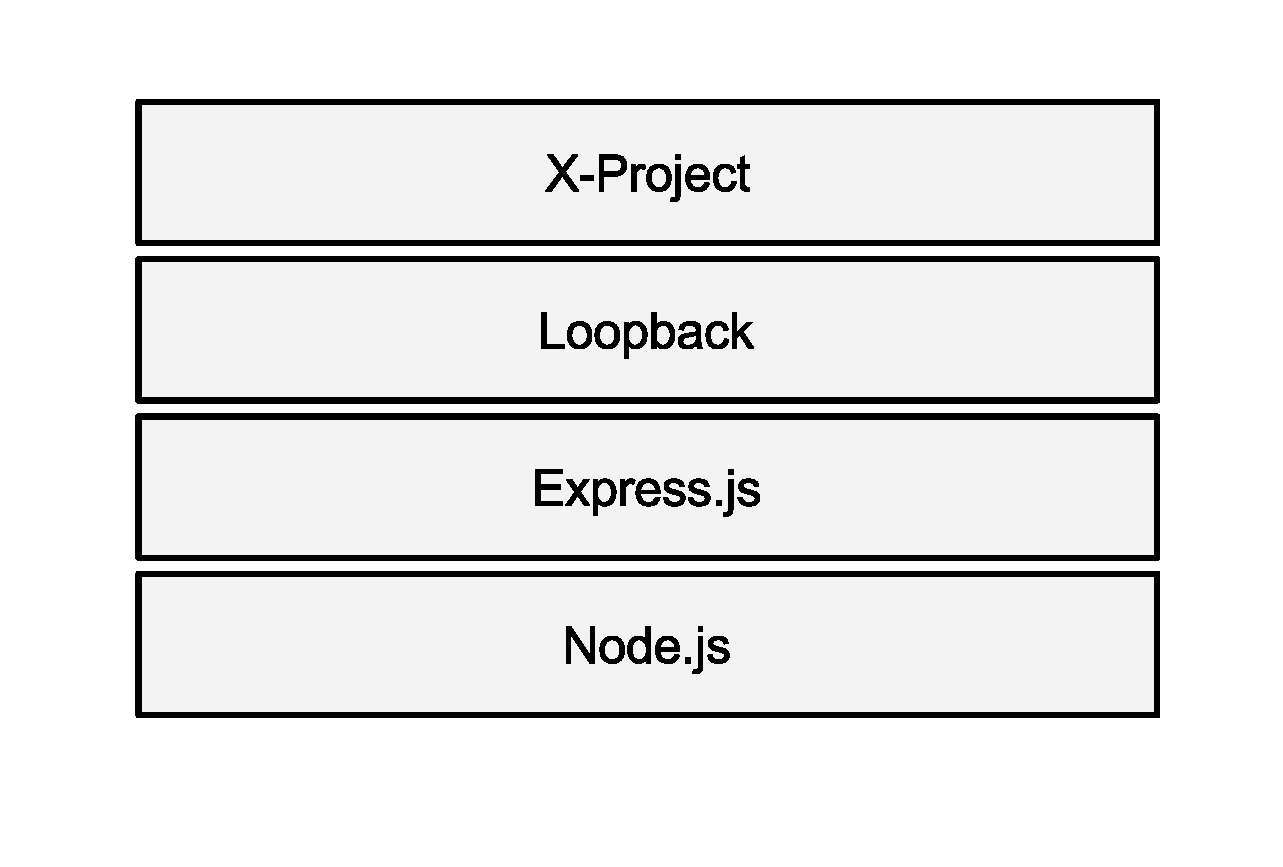
\epsfig{file=images/stack.eps, height=0.2\textwidth}
% \caption{Technology stack}
% \label{fig:tech-stack}
% \end{figure}

% \begin{figure}[!h]
%  \centering
%  \begin{subfigure}[b]{0.53\linewidth}
%  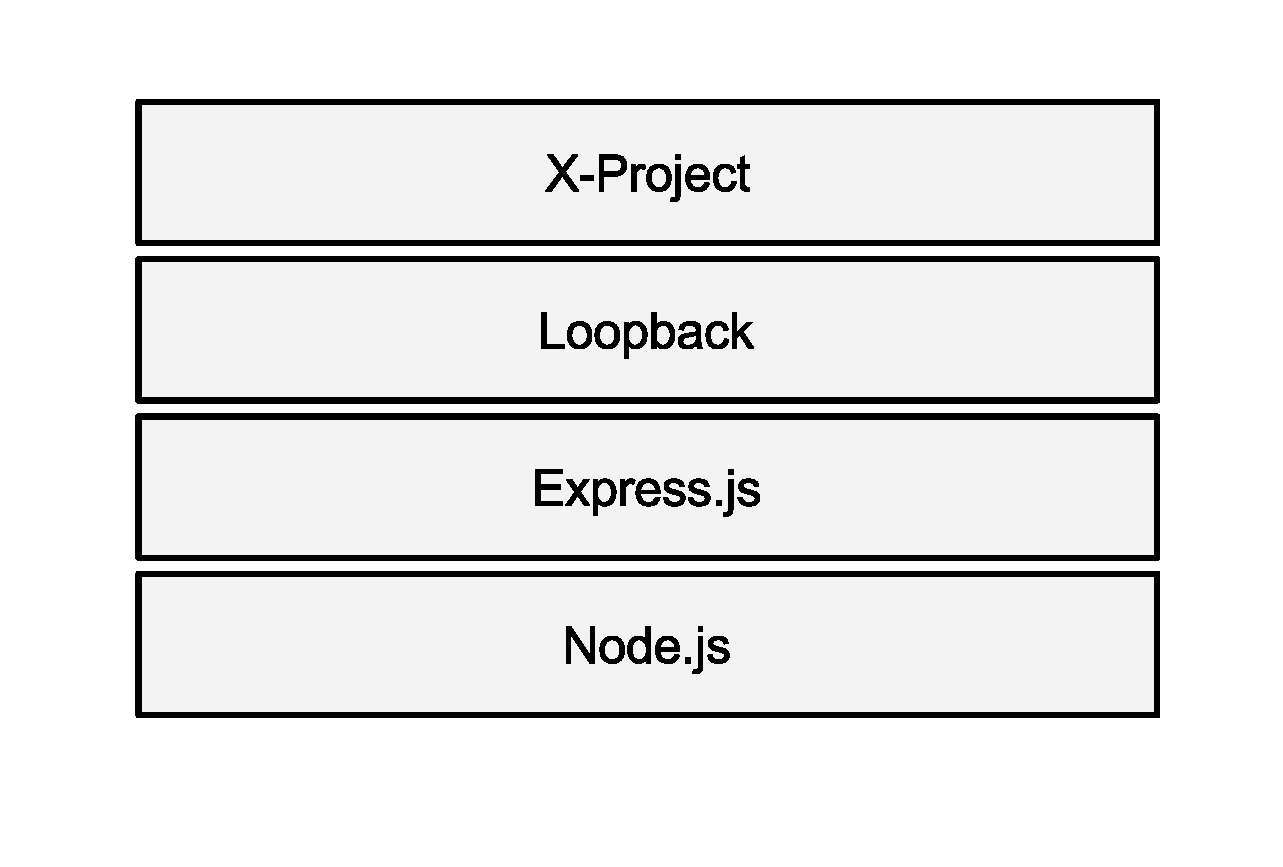
\includegraphics[width=\textwidth]{images/stack.eps} 
%  \caption{Technology stack.}
%  \label{fig:tech-stack}
%  \end{subfigure}
%  ~
%  \begin{subfigure}[b]{0.43\linewidth}
%  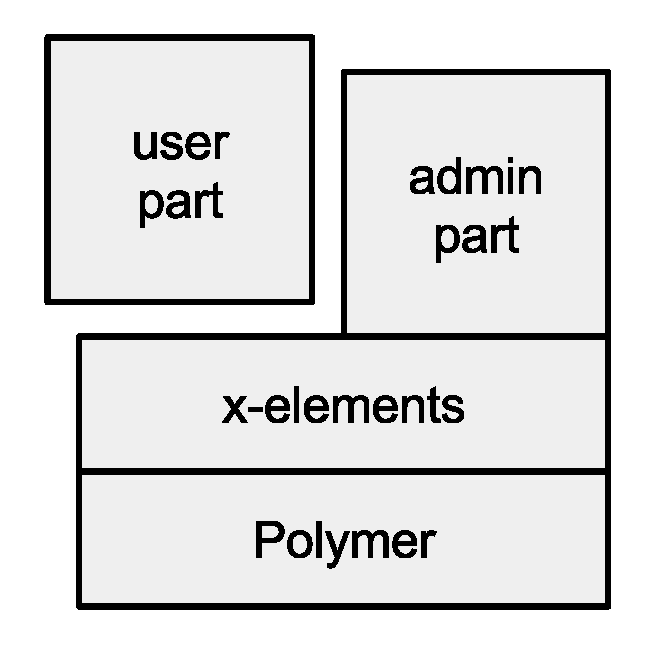
\includegraphics[width=\textwidth]{images/client-arch.eps}
%  \caption{Client-side architecture}
%  \label{fig:client-arch}
%  \end{subfigure}
 
%  % \caption{Office building: 
%  % (a) the schematic plan; 
%  % (b) the simplified 3D model generated for testing on the field 
%  % the indoor mapping project described in this paper.
%  % }
%  % \label{fig:sogei}
% \end{figure}

% \begin{figure}[!htbp]
% \centering
% 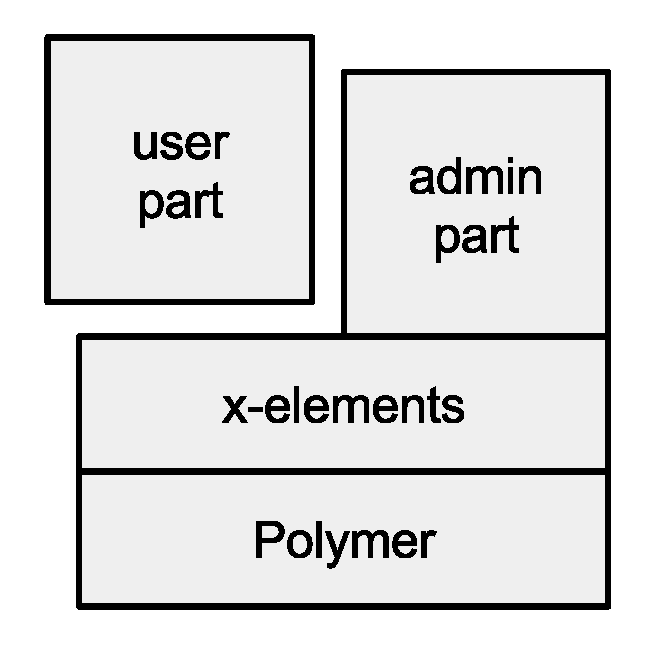
\epsfig{file=images/client-arch.eps, height=0.2\textwidth}
% \caption{Client-side architecture}
% \label{fig:client-arch}
% \end{figure}


\subsection{Server-side}
The Web Application development is document-driven.

To speed up web application development, frameworks mostly rely on external configuration files and less on procedural code \cite{6859693}.


In \brand{x-project}, server-side, the documents that drive the development are the schema of the models of the application.


These are json document. Each document represent a model and has the following fields: the \texttt{name} of the model, the set of \texttt{properties}, the list of \texttt{relations} to others models and the list of \texttt{ACL} (Access Control Layer) rules. 

\brand{x-project} (using Loopback) generates model’s API from the models schemas, to let CRUD operations on models (e.g. a model \texttt{Author} that describe a blog author generates the following HTTP RESTful API: \texttt{GET /api/authors/} to get all authors, \texttt{POST /api/authors/} to add a new author, \texttt{GET /api/authors/:author\_id} and \texttt{PUT /api/authors/:author\_id} to get (or to update) the author with id ``\texttt{author\_id}''. 
Since an blog author have blog posts (its model has a relation one-to-many to model \texttt{Post}) there are also the API to handle author's posts: \texttt{GET /api/authors/:author\_id/posts}, etc.

The API can be extended: the developer can add remote functions to models or add hooks to existing APIs to add behaviour before and/or after the API handler (to preprocess the request and/or postprocess the response).

The API are RESTful, cookie free, signed by authentication token.

\brand{x-project} applications have a built-in model that represent a user, with properties \texttt{username}, \texttt{email} and \texttt{password} for login and the property \texttt{role} used by the ACL module.
By default, only user with role \texttt{admin} can create/update/delete models in the applications.


\subsubsection{Third party services}
\brand{x-project} is designed to be connected to microservices. These tools are accessible extending the Web Application API.

An essential feature of a CMS is media storage (documents, images and videos) \cite{5552271}. 

\brand{x-project} provides a remote storage service implemented as a direct upload module to AWS Amazon S3 storage service. The media to upload don’t pass through the server but are sent directly to AWS using a signed request.
The signature of the request is provided by the module.
The module has to be configured with the AWS bucket settings: bucket name, public and secret keys. 

% \begin{figure}[!htbp]
% \centering
% 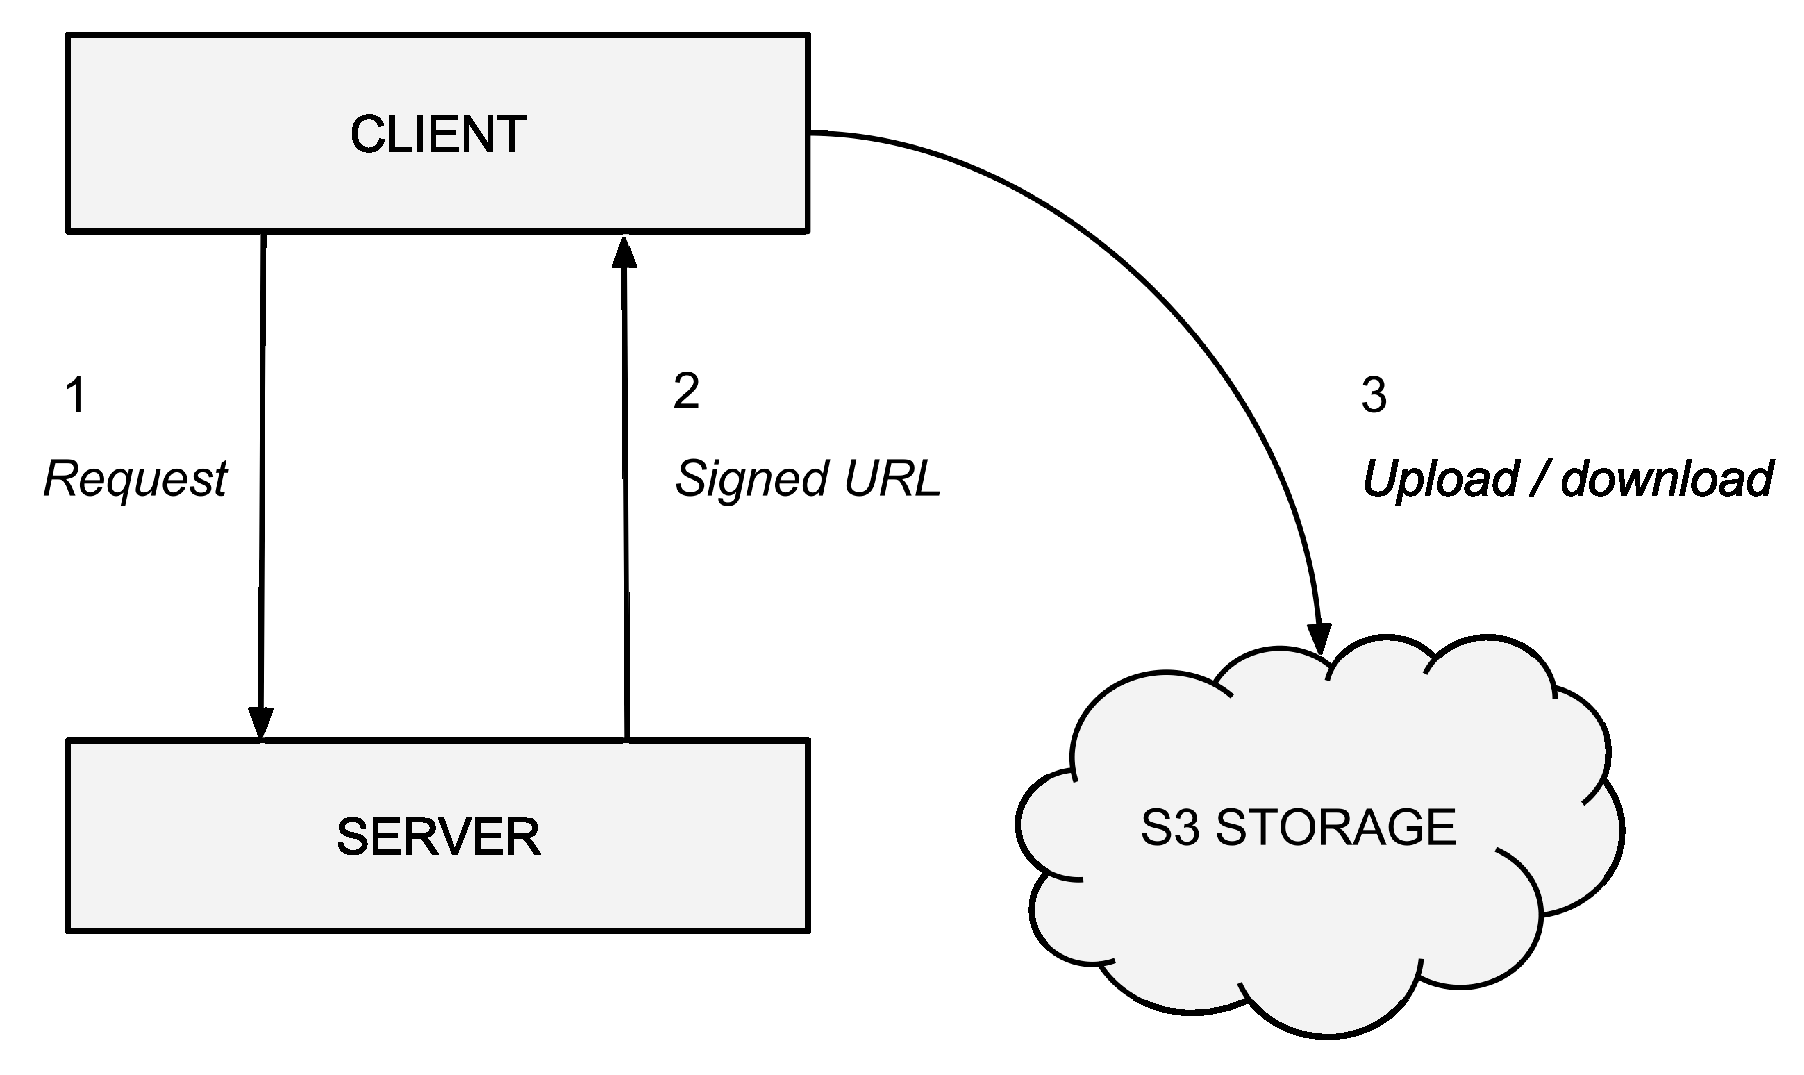
\epsfig{file=images/services.eps, height=0.24\textwidth}
% \caption{Third parties services}
% \label{fig:services}
% \end{figure}


\section{x-project toolkit}\label{sec:toolkit}

``Everything is an element'', from an AJAX request to an entire web page. Every part of the website is encapsulated inside an element. 

\brand{x-project} provide a set of Polymer element for local routing, API requests, forms, lists, and style, as listed below \footnote{\scriptsize For the sake of conciseness, Polymer Elements are presented as empty elements, although empty element type is not supported. Furthermore, template variable are enclosed in single curly brackets while Polymer requires double curly brackets.}. 

Elements can be customized through their attributes. Attributes can acts as inputs parameters (values that have effects to the element) or output parameters (values that are returned by the element).
Values in parameters could be hard-coded (if they never change) or stored in variables.
Different parameters in different elements could use the same variable, so, the value of an output parameter of an element could be used as input in an input parameter of another element.

\paragraph{Elements for local routing}

The following elements performs local routing (for Single Page Application).

\vspace{0.2cm}

\texttt{<x-router>} implements local routing using \emph{HTML5 Push State API}. It represent the core element of the app. It intercepts routes, create pages, and pass parameters to the page.

\vspace{0.2cm}

\texttt{<x-route>} represents a route-to-page mapping. 
Parameters presented in an URL are sent as attributes to the corresponding page.

\begin{lstlisting}[language=HTML5]
<x-route route="{route}" page="{page}" />
\end{lstlisting}

\texttt{<x-link>} is an extension of the anchor element \texttt{<a>} that prevents the default behavior when a click event occurs, blocking page request to the server and redirecting the request to the local router. 

\begin{lstlisting}[language=HTML5]
<a is="x-link" href="{href}">{link}</a>
\end{lstlisting}

\paragraph{Elements for API management}

The following elements handle HTTP RESTful API for the collections of the app.

\texttt{<api-collection-schema>} gets the schema of a collection. 

\begin{lstlisting}[language=HTML5]
<api-collection-schema name="{collection}" 
  schema="{schema}" />
\end{lstlisting}

\vspace{0.2cm}

\texttt{<api-collection-post>} create a model of a collection. 

\begin{lstlisting}[language=HTML5]
<api-collection-post 
  name="{name}" model="{model}" />
\end{lstlisting}

\vspace{0.2cm}

\texttt{<api-collection-get>} gets models of a collection. 

\begin{lstlisting}[language=HTML5]
<api-collection-get 
  name="{collection}" where="{where}" 
  page="{page}" perpage="{perpage}"  
  items="{items}" count="{count}" />
\end{lstlisting}

Where: 
\texttt{name} is the name of the collection to retrieve; 
\texttt{where} is an object that specifies a set of logical conditions to match, similar to a \texttt{WHERE} clause in a SQL query;
\texttt{page} and \texttt{perpage} are parameters for the pagination;
\texttt{items} are the retrieved models that match the query composed by the \texttt{where} clause and the pagination parameters;
\texttt{count} is the size of the collection (the total number of items of the collection).

\vspace{0.2cm}

\texttt{<api-collection-where>} dynamically generates a form from a model schema, to create an API \texttt{where} clause filter. Specifically, for each property described in the model schema, it generates a corresponding input filter field. 

\begin{lstlisting}[language=HTML5]
<api-collection-where schema="{schema}"
  where="{where}" />
\end{lstlisting}

\texttt{<api-model-get>} retrieve a model of a collection. 

\begin{lstlisting}[language=HTML5]
<api-model-get name="{name}" model-id="{id}" 
  model="{model}" />
\end{lstlisting}

Where: 
\texttt{name} is the name of the collection of the model; 
\texttt{model-id} is the model id; 
\texttt{model} is the model retrieved (it acts as an output).

\texttt{<api-model-put>} update a model of a collection. 

\begin{lstlisting}[language=HTML5]
<api-model-put name="{name}" model-id="{id}" 
  model="{model}" />
\end{lstlisting}

Where: 
\texttt{model} is the model updated (it acts as an input).

\vspace{0.2cm}

\texttt{<api-model-del>} delete a model of a collection. 

\begin{lstlisting}[language=HTML5]
<api-model-del name="{name}" model-id="{id}" />
\end{lstlisting}

\paragraph{Elements for forms}
The following elements are used to create forms. 

\vspace{0.2cm}

\texttt{<x-input>} is an extension of the input element. 

\begin{lstlisting}[language=HTML5]
<x-input type="{type}" label="{label}"
  value="{value}" />
\end{lstlisting}

Where: 
\texttt{type} can be \texttt{string}, \texttt{number}, \texttt{date}, \texttt{email}, \texttt{url}, \texttt{location} (with auto-completion based on Google Place API) and \texttt{file}.

\vspace{0.2cm}

\texttt{<x-form>}  dynamically generates a form from a model schema, to create/update a model.

\begin{lstlisting}[language=HTML5]
<x-form schema="{schema}" model="{model}" />
\end{lstlisting}

\paragraph{Elements for lists}

The following elements are used to manage lists. 

\vspace{0.2cm}

\texttt{<x-table>}  dynamically generates a table of models from a model schema. 

\begin{lstlisting}[language=HTML5]
<x-table schema="{schema}" items="{items}" />
\end{lstlisting}

Where \texttt{schema} is used to generate the columns of the table; 
\texttt{collection} is used to generate the rows (the values) of the table.

\vspace{0.2cm}

\texttt{<x-pager>} generate the list of links to handle pagination.

\begin{lstlisting}[language=HTML5]
<x-pager perpage="{perpage}" count="{count}" 
  current="{page}" />
\end{lstlisting}

Where \texttt{count} is the total number of items to paginate; 
\texttt{perpage} is the number of items per page; 
\texttt{current} is the current page selected by the user.

By itself pagination doesn't paginate any list, but it can be used in conjunction with \texttt{<api-collection-get>} (as shown in the case study), where the \texttt{current} output parameter of \texttt{<x-pager>} is the input \texttt{page} parameter of \texttt{<api-collection-get>}.

\paragraph{Elements for style}

The style is based on \texttt{iron-flex-layout} \cite{iron-elements}, a CSS library of style mixins for cross-platform Flexible Box layouts.

\paragraph{Elements for admin pages}

Even a page can be encapsulated in an element. \brand{x-project} provides a set of pages for the admin part of the app, \texttt{<page-collection>} and \texttt{<page-model-edit>}, presented below.

% \begin{figure}[!htbp]
% \centering
% 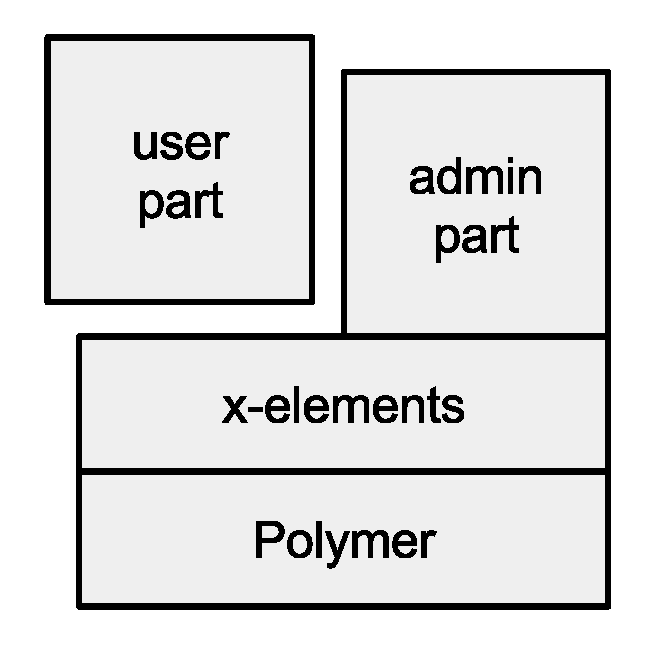
\epsfig{file=images/client-arch.eps, height=0.2\textwidth}
% \caption{Client-side architecture}
% \label{fig:client-arch}
% \end{figure}



\section{Case study}
In this section we discuss the design and the implementation of a blog platform. 

\subsection{server-side}
For a blog platform the entities to model are: \texttt{Author}, \texttt{Post} and \texttt{Tag}.

\texttt{Post} model (defined below) represent a blog post.

\begin{lstlisting}[language=json]
{
  "name": "Post",
  "properties": {
    "title": { "type": "string" },
    "posted": { "type": "date" },
    "content": { "type": "text" },
  }, 
  "relations": [{ 
    "name": "author", 
    "type": "belongs_to",
    "model": "Author",
  }, {
    "name": "tags", 
    "type": "has_many",
    "model": "Tag",
  }]
}
\end{lstlisting}

\texttt{Tag} model represent a tag in a post.

\texttt{Author} model represent a blog author. It has properties that describe an author, such as \texttt{full\_name}, and one \texttt{has\_many} relation to \texttt{Post} model.

  
\subsection{client-side}
Client-side pages are encapsulated in elements that extend \texttt{<x-page>} element. These pages can be divided in two parts: Admin and User.

\subsubsection{Admin part}
The \emph{Admin part} is automatically generated. 
It consists of the following pages: \texttt{<page-collections>}, \texttt{<page-collection>}, \texttt{<page-model-edit>}.

\vspace{0.2cm}

\texttt{<page-collections>} is the main page. It show the collections of the app. In this case, these are \texttt{Authors}, \texttt{Posts} and \texttt{Tag}.

\vspace{0.2cm}

\texttt{<page-collection>} show the model instances of a collection.

\begin{lstlisting}[language=HTML5]
<page-collection>
  <api-collection-get 
    name="{{collection_name}}" 
    filter="{{filter}}"
    collection="{{collection}}">
  </api-collection-get>
  <part-collection-filter 
    name="{{collection_name}}"  
    filter="{{filter}}">
  </part-collection-filter>
  <part-list 
    list="{{collection}}">
  </part-list>
  <part-paginator 
    list="{{list}}" 
    filter="{{filter}}"
    current="{{page}}">
  </part-paginator>
</page-collection>
\end{lstlisting}

\vspace{0.2cm}

\texttt{<page-model-edit>} presents the forms to update a model.
The form is automatically generated from the model schema.
This page is composed by an \texttt{<api-model-get>} element that retrieve the model to edit. The model schema (retrieved with the model) is passed to a \texttt{<x-form>} element that presents an input element for each property of the model. The type of the input element corresponds to the type of the property (e.g. a \emph{boolean} property is editable via a \texttt{<x-checkbox>} element).

\subsubsection{User part}
The \emph{User part} must be designed by the developer.
It consists of the following pages: \texttt{<page-author>}, \texttt{<page-posts>} and \texttt{<page-post>}. 

\vspace{0.2cm}

\texttt{<page-posts>} show the list of posts. It use \texttt{<api-collection-get>}, \texttt{<x-paginator>}, and \texttt{<x-list>} to retrieve, paginate and list the posts.

\vspace{0.2cm}

\texttt{<page-post>} show a post. It is accessible via 
\texttt{<x-route path="/posts/:post\_id" page="page-post">}. It use \texttt{<api-model-get>} to retrieve the post using the \texttt{post\_id} parameter matched in the url.

\begin{lstlisting}[language=HTML5]
<page-post>
  <api-model-get name="Posts" 
    model-id="{{post_it}}" model="{{post}}">
  </api-model-get>
  <h1>{{post.title}}</h1>
  <h2>by {{post.author}}</h2>
  <h3>on {{post.date}}</h3>
  <div>{{post.content}}</div>
</page-post>
\end{lstlisting}


\section{Document-driven web development process}\label{sec:dev-proc}

It is possible to outline the activities performed in the case-study to elicit a development approach that imposes a neat logic decomposition that strongly supports an engineeared design of the web application. The identified main acitivities can be arranged in the following four subsequential steps.

{\bf 1\textsuperscript{st} step - JSON documents definintion}. The input JSON documents must be defined specifying data model schemas, model relations, user roles read/write capabilities on particular portion of data, and ancillary configurations (e.g. DBMS type). The output of this stage is a comprehensive set of HTTP RESTfull API to operate CRUD methods on defined data.

{\bf 2\textsuperscript{nd} step - Model actions definion}. Further actions on models besides CRUD ones must be defined in this step and exposed as RESTful API via HTTP verbs.

{\bf 3\textsuperscript{rd} step - UI component definition}. Distinct UI component must be defined, or retrieved from a collection of predefined components, configurated and adapted. As concerns server communication, these components may avail only of the HTTP RESTfull API defined in the previous two steps.

{\bf 4\textsuperscript{th} step - UI component assemblation}. Distinct UI components are finally mounted to compose the application views. Assembly is kept as simple as possible: it only consists of a composition of HTML5 elements.


% This modellization is based on the reasonable assumption that server side
% operation on data models are nowadays be sufficently explored, and as proven by
% the {\em KeystoneJS} experience, at least one choice is available to automagically  
% 1) generate server-side CRUD methods on models with ACL capabilities and 
% 2) handle users and sessions, 
% once a JSON description of data models and relations between them are provided to the
% system. This very JSON descriptor documents drive the whole process, actually composed
% by the following four steps.

% se avanza spazio si possono mettere dei nomignoli per ogni stepche potrebbero essere:
% 1. JSON data model description
% 2. Model actions definion
% 3. UI component definition
% 4. UI component assemplation

% PARLARE DI DECOMPOSIZIONE VERTICALE??


%\section{Conclusion}\label{sec:conclusions}

In the present time open source CMS has gained a big market. 
Generally all CMSs fulfill common task of content like create, edit, publish. 
Lots of varieties are available based on functionality and platform, such as \emph{good user support}, \emph{security aspects}, \emph{plug-ins ecosystem}, \emph{documentation}, etc.

\cite{6169111} propose different performance criteria like \emph{page load time}, \emph{page size}, \emph{number of request}, \emph{number of bootstrap resources files}.
 
\cite{5552271} propose about thirty features criteria that could be classified in: \emph{Admin Management}, \emph{Data Management}, \emph{User Management}, \emph{UI Management}, \emph{Web Content Management}, \emph{Multimedia Data Management}.



\bibliographystyle{abbrv}
\bibliography{x-project-paper}
\end{document}





